\subsection{Data Injection Position Dense}
If the data injection positions are dense, which means the data injection position connect with each other. 

\vspace*{15pt}

The sun-optimal solution is that

\begin{itemize}
\item we consider the whole cluster data load injection as one data injection 
\item execute the equal power algorithm in chapter one to process the divisible load theory principle.
\item re-balance the load fraction between nodes in the cluster
\end{itemize}

Consider the Fig.\ref{dense1}

\vspace*{15pt}

\begin{figure}[h]
\centering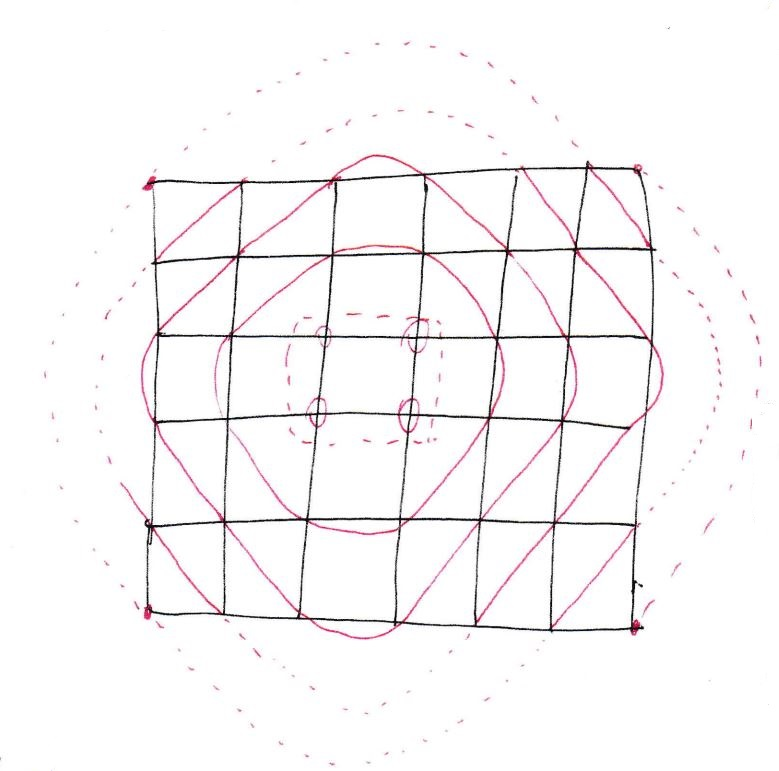
\includegraphics[width=0.8\linewidth]{figure/dense1}
\caption{4 data injection connecting with each other consists of a whole cluster}
\label{dense1}
\end{figure}

The equal power matrix with front end as follows:

\begin{equation}
{
\left[ \begin{array}{ccccc}
4 & 8 & 10 & 6 & 2 \\
1 & -1 & 0 & 0 & 0\\
0 & \sigma -1 & 1 & 0 & 0  \\
0 & \sigma -1 & \sigma & 1 & 0  \\
0 & \sigma -1 & \sigma & \sigma & 1  \\
\end{array} 
\right ]}  
\end{equation}


The equal power matrix without front end as follows:

\begin{equation}
{
\left[ \begin{array}{ccccc}
4 & 8 & 10 & 6 & 2 \\
1 & {\sigma}^{\star} & 0 & 0 & 0 \\
1 & -\sigma & {\sigma}^{\star} & 0 & 0  \\
1 & -\sigma & -\sigma & {\sigma}^{\star} & 0  \\
1 & -\sigma & -\sigma & -\sigma & {\sigma}^{\star}\\

\end{array} 
\right ]} 
\end{equation}

\vspace*{50pt}

Consider the Fig.\ref{dense2}
\begin{figure}[h]
\centering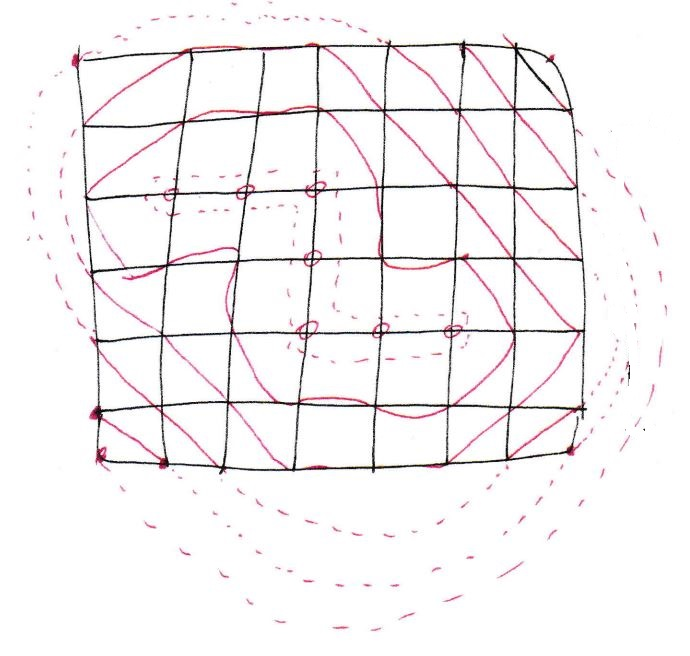
\includegraphics[width=0.8\linewidth]{figure/dense2}
\caption{7 data injection connecting with each other consist of a whole cluster}
\label{dense2}
\end{figure}

\vspace*{20pt}
The equal power matrix with front end as follows:

\begin{equation}
{
\left[ \begin{array}{ccccccc}
7 & 14 & 15 & 10 & 6 & 3 & 1 \\
1 & -1 & 0 & 0 & 0 & 0 & 0\\
0 & \sigma -1 & 1 & 0 & 0 & 0 & 0 \\
0 & \sigma -1 & \sigma & 1 & 0 & 0 & 0 \\
0 & \sigma -1 & \sigma & \sigma & 1 & 0 & 0 \\
0 & \sigma -1 & \sigma & \sigma & \sigma & 1 & 0 \\
0 & \sigma -1 & \sigma & \sigma & \sigma & \sigma & 1 \\
\end{array} 
\right ]}  
\end{equation}

\vspace*{20pt}
The equal power matrix without front end as follows:

\begin{equation}
{
\left[ \begin{array}{ccccccc}
7 & 14 & 15 & 10 & 6 & 3 & 1 \\
1 & {\sigma}^{\star} & 0 & 0 & 0 & 0 & 0 \\
1 & -\sigma & {\sigma}^{\star} & 0 & 0 & 0 & 0 \\
1 & -\sigma & -\sigma & {\sigma}^{\star} & 0 & 0 & 0 \\
1 & -\sigma & -\sigma & -\sigma & {\sigma}^{\star} & 0 & 0\\
1 & -\sigma & -\sigma & -\sigma & -\sigma & {\sigma}^{\star}  & 0\\
1 & -\sigma & -\sigma & -\sigma & -\sigma & -\sigma & {\sigma}^{\star}\\

\end{array} 
\right ]} 
\end{equation}

So this kind of problem is transfered to finding the number of node on each level(contour line).

\vspace*{50pt}
\subsection{Choosing The Data Load Position}
The data injection position are affected by two factors. 

\begin{itemize}
\item the distance between each data load injection
\item the number of unit cores in its Voronoi cell community.
\end{itemize}

So we choose the Manhattan distance centroidal voronoi tessellations\cite{du1999centroidal} to choose the data injection position.
\\
For example, we consider the 80*80 regular mesh, we have 10 data injection budget to choose 10 appropriate position.

We can see the simulation result from Fig.\ref{cvt1} and Fig.\ref{cvt20}
\vspace*{20pt}

\begin{figure}[h]
\centering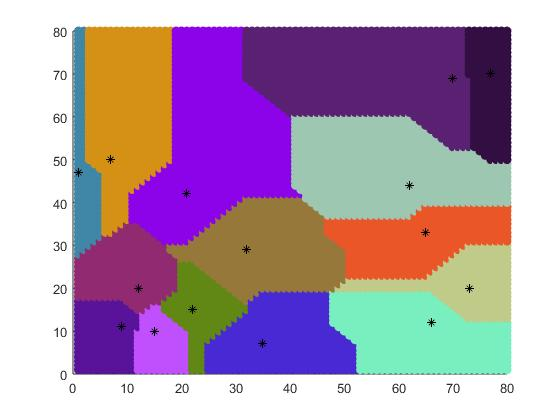
\includegraphics[width=0.8\linewidth]{figure/cvt1}
\caption{Random choose 10 potential position to do the community division }
\label{cvt1}
\end{figure}

\begin{figure}[h]
\centering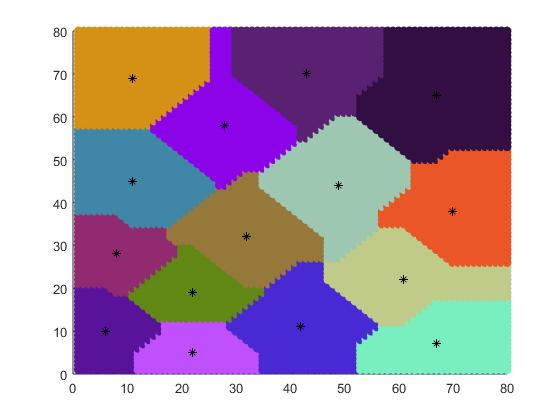
\includegraphics[width=0.8\linewidth]{figure/cvt20}
\caption{After 20 rounds the division achieve stable}
\label{cvt20}
\end{figure}

\subsection{Re-balance the community division }

Considering the speedup ability depends on the number of short distance unit core.
So after $1000$ times random experiment, we find we can achieve the same computation ability yet save over $30\%$ unit core.

\vspace*{20pt}
\textbf{
The principle is we choose the minimum value of the largest depth of each community as the depth rule.}

$$L =  min(max(voronoi \quad cell \quad depth))$$

\vspace*{20pt}

One example Fig.\ref{voronoi} Fig.\ref{voronoisave} presents:
\\

\begin{figure}[h]
\centering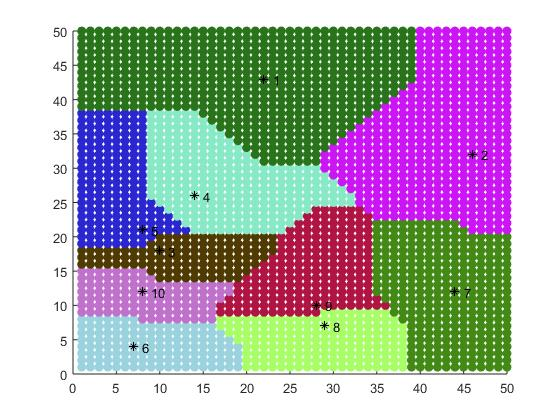
\includegraphics[width=0.8\linewidth]{figure/voronoi}
\caption{50*50 regular mesh with 10 division cell}
\label{voronoi}
\end{figure}

\begin{figure}[h]
\centering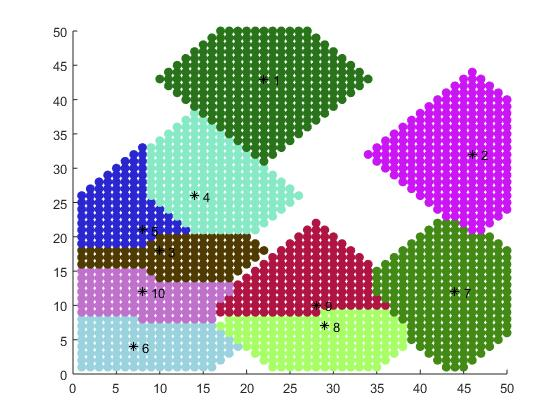
\includegraphics[width=0.8\linewidth]{figure/voronoisave}
\caption{50*50 regular mesh with 10 division cell and save over 30\% unit core}
\label{voronoisave}
\end{figure}

We also can find the speedup result from figures Fig.\ref{voronoicurve} and Fig.\ref{voronoisavecurve}:
\\
\begin{itemize}
\item $\sigma < 0.2$ the ratio is $5$. Fig.\ref{voronoicurve}
\item after re-balance the ratio is about $2.7$ \ref{voronoisavecurve}
\end{itemize}

\begin{figure}[h]
\centering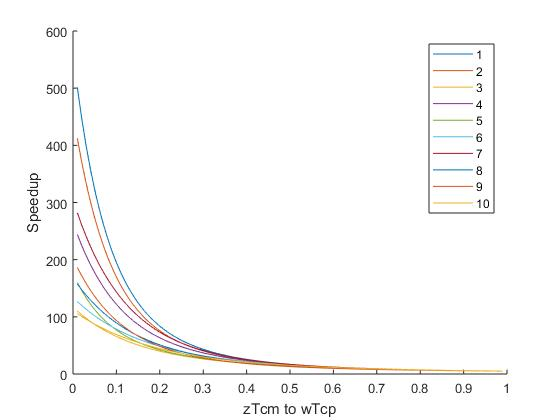
\includegraphics[width=0.8\linewidth]{figure/voronoi_curve}
\caption{50*50 regular mesh with 10 division cell}
\label{voronoicurve}
\end{figure}

\begin{figure}[h]
\centering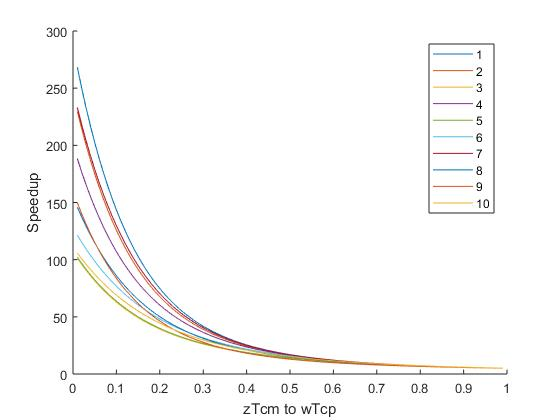
\includegraphics[width=0.8\linewidth]{figure/voronoi_curve2}
\caption{50*50 regular mesh with 10 division cell}
\label{voronoisavecurve}
\end{figure}












